%!Mode::"UTF-8"
\documentclass[12pt]{article}

% 页面设置
\usepackage{geometry}
\geometry{left=2.5cm, right=2.5cm, top=2.5cm, bottom=2.5cm}
\usepackage{graphicx}
\usepackage{ctex}
\usepackage{fontspec}
\usepackage{setspace}

% 代码设置
\usepackage{listings}
\usepackage{color}
\setmonofont{Consolas}
\definecolor{listing}{gray}{0.97}
\lstset{
	backgroundcolor=\color{listing},
	basicstyle=\footnotesize,
	numbers=left,
	numberstyle=\footnotesize,
	stepnumber=1,
	aboveskip={0.5\baselineskip},
	belowskip={0.5\baselineskip},
	columns=fullflexible,
	breaklines=true,
	breakatwhitespace=true,
	frame=single,
	basicstyle=\ttfamily,
	numberstyle=\ttfamily,
	tabsize=2
}

% 字体设置
\setmainfont{Times New Roman}
\setCJKmainfont{SimSun}
\setCJKsansfont{SimHei}
\usepackage[version=4]{mhchem}

% 表格设置
\usepackage{makecell}
\newcommand{\addcell}[2][4]{\makecell{\zihao{#1}\textsf{#2}}}
\usepackage{titlesec}
\usepackage{booktabs}
\usepackage{tabularx}

% 设置图注、表注
\usepackage{caption}
\usepackage{bicaption}
\captionsetup{labelsep=quad, font={small, bf}, skip=2pt}
\DeclareCaptionOption{english}[]{
    \renewcommand\figurename{Fig.}
    \renewcommand\tablename{Table}
}
\captionsetup[bi-second]{english}

% 设置页眉
\usepackage{fancyhdr}
\pagestyle{fancy}
\fancypagestyle{preContent}{
    \fancyhead[L]{\zihao{-5} 物理化学实验}
    \fancyhead[C]{\zihao{-5} 实验一\ \ 燃烧热的测定}
    \fancyhead[R]{\zihao{-5} 1800011828\ 王宇哲}
}
\pagestyle{preContent}

%	设置首页页眉页脚
\fancypagestyle{plain}{
	\fancyhead[L]{\zihao{-5} 物理化学实验}
	\fancyhead[C]{\zihao{-5} 实验一\ \ 燃烧热的测定}
	\fancyhead[R]{\zihao{-5} 1800011828\ 王宇哲}
	\cfoot{}
}

% 设置标题格式
\titleformat*{\section}{\zihao{4}\sffamily}
\titleformat*{\subsection}{\zihao{-4}\sffamily}
\titleformat*{\subsubsection}{\zihao{-4}\sffamily}
\titlespacing*{\section}{0pt}{10pt}{10pt}
\titlespacing*{\subsection}{0pt}{10pt}{5pt}
\titlespacing*{\subsubsection}{0pt}{10pt}{5pt}

% 设置引用格式
\usepackage[super,round,comma,compress]{natbib}

\usepackage{amsmath}
\usepackage{amssymb}

%设置封面
\begin{document}
    % 标题页
    \begin{titlepage}
    	% 页眉
    	\thispagestyle{plain}
        % 图片
        \begin{figure}[h]
            \centering
            \includegraphics{pku.png}
        \end{figure}
        \vspace{24pt}
        % 标题
        \centerline{\zihao{-0} \textsf{物理化学实验报告}}
        \vspace{40pt} % 空行
        \begin{center}
            \begin{tabular}{cp{6 cm}}
                % 题目
                \addcell[2]{题目:\ } & \addcell[2]{燃烧热的测定} \\
                \cline{2-2}
            \end{tabular}
        \end{center}
        \vspace{20pt} % 空行
        \begin{center}
            \doublespacing
            \begin{tabular}{cp{5cm}}
                % 姓名
                \addcell{姓\phantom{空格}名:\ } & \addcell{王宇哲} \\
                \cline{2-2}
                % 学号
                \addcell{学\phantom{空格}号:\ } & \addcell{1800011828}\\
                \cline{2-2}
                % 组别
                \addcell{组\phantom{空格}别:\ } & \addcell{11组3号} \\
                \cline{2-2}
                % 实验日期
                \addcell{实验日期:\ } & \addcell{2020.12.16}\\
                \cline{2-2}
                % 室温
                \addcell{室\phantom{空格}温:\ } & \addcell{291.75\ K}\\
                \cline{2-2}
                % 大气压强
                \addcell{大气压强:\ } & \addcell{103.17\ kPa}\\
                \cline{2-2}
            \end{tabular}
            \begin{tabular*}{\textwidth}{c}
                \\ % 这是空行
                \\ % 这是空行
                \\ % 这是空行
                \\ % 这是空行
                \hline % 分割线
            \end{tabular*}
        \end{center}
        % 摘要
        \textsf{摘\ \ 要}\ \ 本实验通过氧弹式量热计中苯甲酸和蔗糖的恒容燃烧,经雷诺校正及热力学计算得到量热计常数$W=(2.40\pm 0.09)\ \ {\rm kJ\cdot K^{-1}}$,蔗糖的恒容燃烧热及恒压燃烧热$Q_{P}=Q_{V}=-(16.5\pm 0.2)\ \ {\rm kJ\cdot g^{-1}}$,换算得$\Delta_{c}H_{m}=-(5648\pm 64)\ \ {\rm kJ\cdot mol^{-1}}$,与文献值的偏差$\xi=0.12\%$,并对加入水量误差、实验条件偏离标准态误差、固体脱落误差等进行了分析。
        \\
        \\
        % 关键字
        \textsf{关键词}\ \ 燃烧热;氧弹式热量计;雷诺校正
    \end{titlepage}

    \section{引言}
	略
               
\vbox{}        
    \section{实验部分}
    	\subsection{仪器和试剂}
    	苯甲酸(AR),蔗糖(AR),去离子水。\par 
    	百分之一天平,分析天平,压片机,RF-K1型氧弹式热量计,万用表,$\rm SWC-II_{D}$型精密数字温度温差测量仪,棉线,镍丝,$\rm 2000 \ \ {\rm mL}$容量瓶,$\rm 1000 \ \ {\rm mL}$容量瓶,研钵及研杵。
     
\vbox{}
    	 \subsection{实验内容\citealp{physchemlab}}
			\subsubsection{水当量(量热计常数)的测量}
		取$\sim 0.92\ \ {\rm g}$苯甲酸,置于压片机中压成圆柱体。取出后,用$\sim 15\ \ {\rm cm}$长、用分析天平精确称量其质量为$m^{\prime}=0.0164\ \ {\rm g}$的棉线将圆柱体样品系好,用分析天平精确称量其质量为$m=0.9208\ \ {\rm g}$,则样品质量$m-m^{\prime}=0.9044\ \ {\rm g}$。\par 
		取$\sim 10\ \ {\rm cm}$长、用分析天平精确称量其质量为$m_{0}=0.0103\ \ {\rm g}$的燃烧丝,将两端分别紧缠在电极A和电极B上,再将已被棉线缠系的圆柱体状样品用棉线系在燃烧丝上,小心挂在燃烧皿中。盖好弹盖,从进气口灌入$\sim 1\ \ {\rm MPa}$的氧气,洗气3次,排尽氧弹里的空气,最后灌入$1\ \ {\rm MPa}$氧气后,用万用表表笔触试弹头和进气阀体,测量氧弹电阻$\sim 4.50\ \ \Omega$,符合要求。\par 
		用$2000\ \ {\rm mL}$容量瓶准确量取$2000\ \ {\rm mL}$室温去离子水,顺筒壁小心倒入内筒。把氧弹放入内筒,再用$1000\ \ {\rm mL}$容量瓶准确量取$1000\ \ {\rm mL}$室温去离子水倒入内筒。盖好盖板,插上温差仪插头,开动搅拌马达。待水温稳定后,打开秒表作为开始时间,记录体系温度随时间变化情况。$3\sim 5\ \ {\rm min}$后,按下点火键$2\sim 3\ \ {\rm s}$,使苯甲酸燃烧,$15\ \ {\rm s}$读取温度一次,直至每次读数时温度上升$<0.1\ \ {\rm ^{\circ}C}$。待温度稳定变化时,$3\sim 5\ \ {\rm min}$后停止搅拌,小心取下温差仪探头,取出氧弹,在通风橱里泄去废气,旋开弹盖,取出弹头,称量剩余燃烧丝质量为$m_{1}=0.0089\ \ {\rm g}$。
		
		
\subsubsection{蔗糖燃烧热的测量}
	以同样的方法测定蔗糖的燃烧热。称量$\sim 1.00\ \ {\rm g}$蔗糖,棉线质量$m^{\prime}=0.0185\ \ {\rm g}$,棉线与样品的总质量$m=0.9862\ \ {\rm g}$,则样品质量$m-m^{\prime}=0.9677\ \ {\rm g}$。燃烧丝初始质量$m_{0}=0.0115\ \ {\rm g}$,测量氧弹电阻$\sim 2.59\ \ \Omega$。蔗糖燃烧热测量结束后,称量剩余燃烧丝质量为$m_{1}=0.0096\ \ {\rm g}$。


 \section{数据与结果}
 \subsection{实验数据记录及处理}
 \subsubsection{水当量(量热计常数)的测量及雷诺校正}
 记录苯甲酸燃烧过程中体系温度相对初始温度的温差$\Delta T$随时间$t$的变化,结果如\textbf{表1}所示。
\begin{table}[h]
	\centering
	\zihao{5}
	\bicaption{苯甲酸燃烧过程体系温度变化实验数据}{Experimental data of temperature change of benzoic acid combustion process}
	\begin{tabular}{ccccccccccc}
		\toprule
		$t/{\rm s}$ & $\Delta T/{\rm ^{\circ}C}$ & & $t/{\rm s}$ & $\Delta T/{\rm ^{\circ}C}$& & 	$t/{\rm s}$ & $\Delta T/{\rm ^{\circ}C}$ & & $t/{\rm s}$ & $\Delta T/{\rm ^{\circ}C}$ \\
		\midrule
		0   & 0.000 &  & 240 & 0.014 &  & 435 & 1.425 &  & 600 & 1.651 \\
		15  & 0.001 &  & 270 & 0.016 &  & 450 & 1.467 &  & 630 & 1.667 \\
		30  & 0.003 &  & 300 & 0.016 &  & 465 & 1.502 &  & 660 & 1.678 \\
		49  & 0.004 &  & 315 & 0.026 &  & 480 & 1.530 &  & 690 & 1.688 \\
		60  & 0.006 &  & 330 & 0.177 &  & 495 & 1.554 &  & 720 & 1.695 \\
		75  & 0.007 &  & 345 & 0.516 &  & 510 & 1.574 &  & 750 & 1.701 \\
		91  & 0.008 &  & 360 & 0.828 &  & 525 & 1.592 &  & 780 & 1.706 \\
		120 & 0.009 &  & 375 & 1.052 &  & 540 & 1.602 &  & 810 & 1.709 \\
		150 & 0.011 &  & 390 & 1.197 &  & 555 & 1.621 &  &     &       \\
		180 & 0.012 &  & 405 & 1.297 &  & 570 & 1.633 &  &     &       \\
		212 & 0.012 &  & 420 & 1.376 &  & 585 & 1.643 &  &     &      \\
		\bottomrule
	\end{tabular}
\end{table}
\par
根据\textbf{表1}数据,作出苯甲酸燃烧过程的温差$\Delta T-$时间$t$散点图,使用python SciPy InterpolatedUnivariateSpline用3次B样条曲线平滑连接各点,作出苯甲酸燃烧过程的$\Delta T-t$曲线,并通过雷诺校正对苯甲酸燃烧过程的体系温度变化进行修正,如\textbf{图1}所示。

\begin{figure}[h]
	\centering
	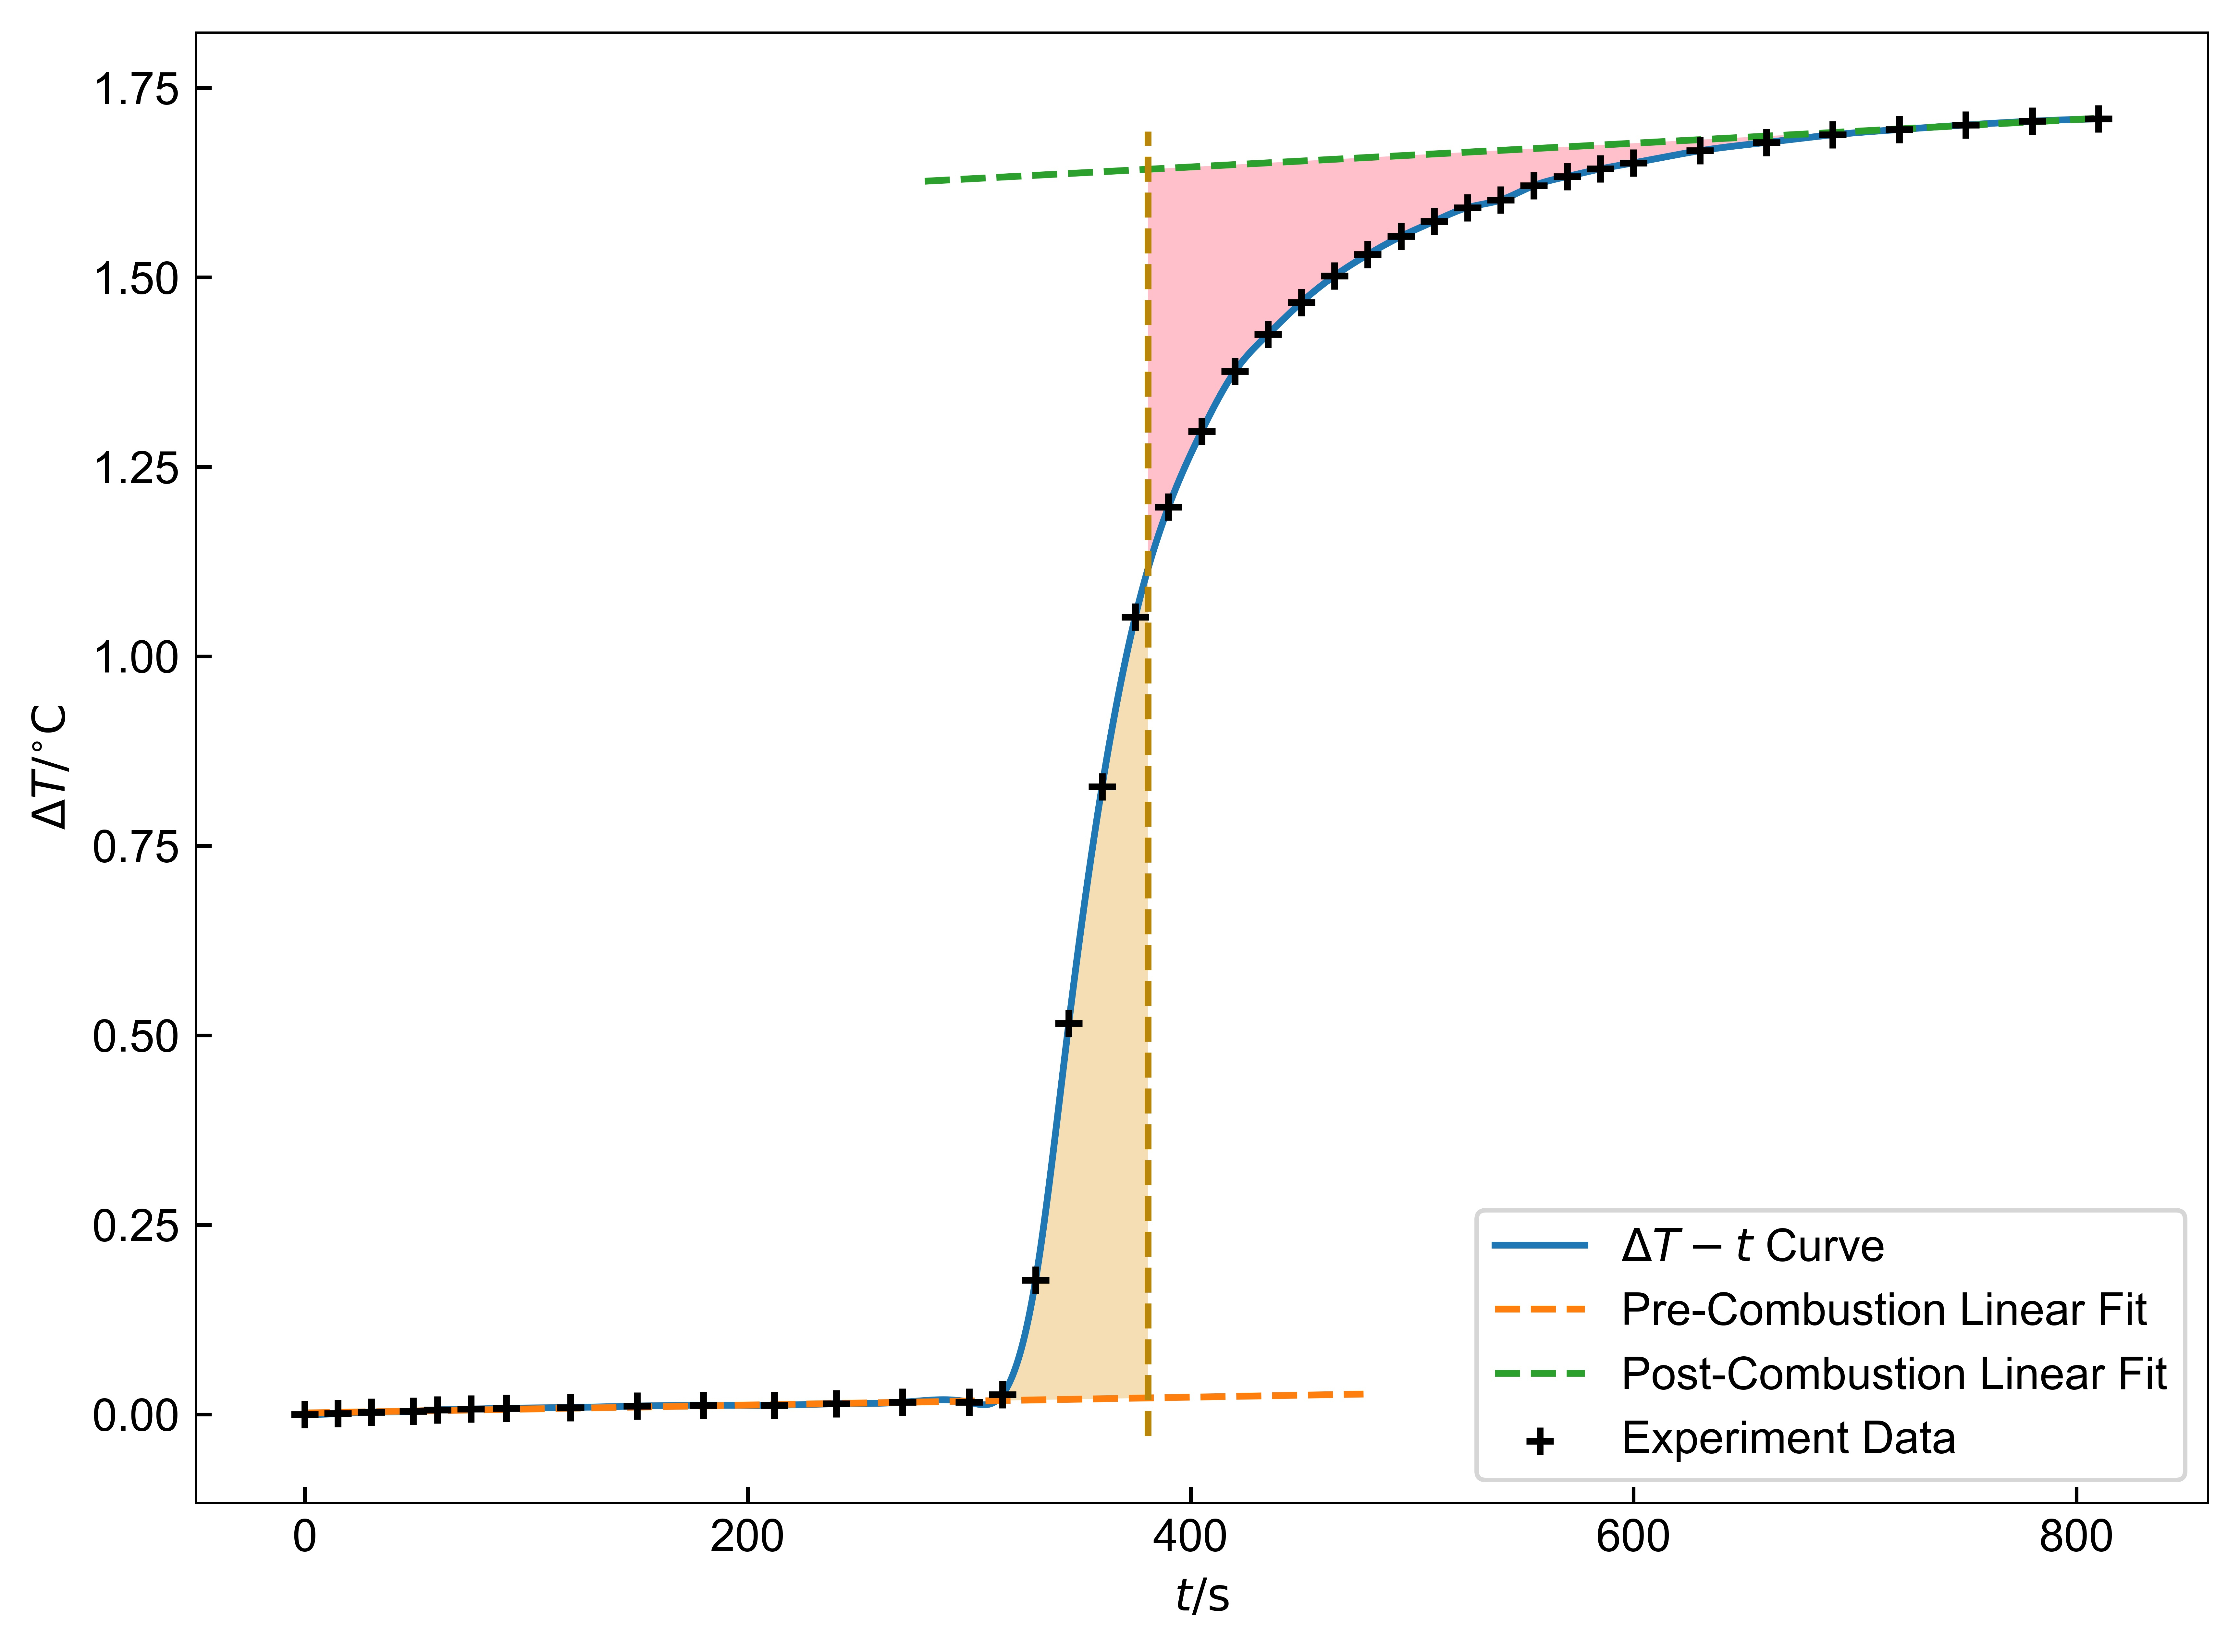
\includegraphics[width=0.7\textwidth]{1.jpg}
	\bicaption{苯甲酸燃烧过程$\Delta T-t$曲线及雷诺校正}{$\Delta T-t$ curve of benzoic acid combustion process and Renolds correction}
\end{figure}
\par

雷诺校正的原理简述如下。在测定燃烧热实验的过程中,体系与环境间不断交换能量。在测定的前期和末期,体系和环境间温差的变化不大,交换能量较稳定;而反应期温度改变较大,体系和环境的温差随时改变,交换的热量也不断改变,很难用实验数据直接求算。进行雷诺校正时,通过作出测定前期和测定末期$\Delta T-t$曲线的切线,作一垂线使其与$\Delta T-t$曲线及两切线包围的两部分面积相等,则垂线与两切线交点的温度差$\Delta T_{0}$即为体系内部燃烧过程放出热量致使体系温度升高的数值。如\textbf{图1}所示,使用python SciPy linregress作出测定前期(苯甲酸燃烧前)和测定末期(苯甲酸燃烧后)实验数据的拟合直线,作为$\Delta T-t$曲线的切线,测定前期拟合直线的方程为
$$
\Delta T/{\rm ^{\circ}C} =(5.2\pm 0.3)\times 10^{-5} \ \ t/{\rm s}+(1.8\pm 0.5)\times 10^{-3},\  \ R^{2}=0.9522
$$
测定末期拟合直线的方程为
$$
\Delta T/{\rm ^{\circ}C} =(1.6\pm 0.2)\times 10^{-4} \ \ t/{\rm s}+(1.58\pm 0.01),\  \ R^{2}=0.9796
$$
\par 
使用python SciPy integrate计算数值积分,求算$\Delta T-t$曲线、垂线与两拟合直线围成的两部分面积(如\textbf{图1}所示,黄色和粉色部分);使用二分法(设定误差$<10^{-10} \ \ {\rm ^{\circ}C\cdot s}$)确定使得两部分面积相等的时间点$t_{0}$,经python程序计算,得到
$$
t_{0}=380.73\ \ {\rm s}
$$
记拟合直线的斜率为$k$,截距为$b$,计算垂线$t=t_{0}$与测定前期拟合直线的交点对应的温差
$$
\Delta T_{1}=k_{1}t_{0}+b_{1}=(5.2\times 10^{-5} \times 380.73+1.8\times 10^{-3})\ \ {\rm ^{\circ}C}=0.022\ \ {\rm ^{\circ}C}
$$
$\Delta T_{1}$的不确定度
$$
\sigma_{\Delta T_{1}}=\sqrt{\sigma^{2}_{k_{1}}t^{2}_{0}+\sigma^{2}_{b_{1}}}=\sqrt{(0.3\times 10^{-5} \times 380.73)^{2}+(0.5\times 10^{-3})^{2}} \ \ {\rm ^{\circ}C}=0.001\ \ {\rm ^{\circ}C}
$$
故
$$\Delta T_{1}=(0.022\pm 0.001)\ \ {\rm ^{\circ}C}
$$
计算垂线$t=t_{0}$与测定末期拟合直线的交点对应的温差
$$
\Delta T_{2}=k_{2}t_{0}+b_{2}=(1.6\times 10^{-4} \times 380.73+1.58)\ \ {\rm ^{\circ}C}=1.64\ \ {\rm ^{\circ}C}
$$
$\Delta T_{2}$的不确定度
$$
\sigma_{\Delta T_{2}}=\sqrt{\sigma^{2}_{k_{2}}t^{2}_{0}+\sigma^{2}_{b_{2}}}=\sqrt{(0.2\times 10^{-4} \times 380.73)^{2}+0.01^{2}} \ \ {\rm ^{\circ}C}=0.01\ \ {\rm ^{\circ}C}
$$
故
$$\Delta T_{2}=(1.64\pm 0.01)\ \ {\rm ^{\circ}C}
$$
因此,计算苯甲酸燃烧过程放出热量致使体系温度升高的数值
$$
\Delta T_{0}=\Delta T_{2}-\Delta T_{1}=1.62\ \ {\rm ^{\circ}C}
$$
$\Delta T_{0}$的不确定度
$$
\sigma_{\Delta T_{0}}=\sqrt{\sigma^{2}_{\Delta T_{1}}+\sigma^{2}_{\Delta T_{2}}}=0.01\ \ {\rm ^{\circ}C}
$$
故
$$
\Delta T_{0}=(1.62\pm 0.01)\ \ {\rm ^{\circ}C}
$$

\subsubsection{蔗糖燃烧热的测量及雷诺校正}
记录蔗糖燃烧过程中体系温度相对初始温度的温差$\Delta T$随时间$t$的变化,结果如\textbf{表2}所示。
\begin{table}[h]
	\centering
	\zihao{5}
	\bicaption{蔗糖燃烧过程体系温度变化实验数据}{Experimental data of temperature change of sucrose combustion process}
	\begin{tabular}{ccccccccccc}
		\toprule
		$t/{\rm s}$ & $\Delta T/{\rm ^{\circ}C}$ & & $t/{\rm s}$ & $\Delta T/{\rm ^{\circ}C}$& & 	$t/{\rm s}$ & $\Delta T/{\rm ^{\circ}C}$ & & $t/{\rm s}$ & $\Delta T/{\rm ^{\circ}C}$ \\
		\midrule
		0   & 0.000  &  & 210 & -0.011 &  & 405 & 0.928 &  & 600 & 1.086 \\
		15  & -0.001 &  & 240 & -0.012 &  & 420 & 0.954 &  & 630 & 1.094 \\
		30  & -0.006 &  & 270 & -0.012 &  & 435 & 0.977 &  & 660 & 1.099 \\
		45  & -0.008 &  & 285 & 0.004  &  & 450 & 0.996 &  & 690 & 1.103 \\
		60  & -0.009 &  & 300 & 0.159  &  & 465 & 1.011 &  & 720 & 1.107 \\
		75  & -0.010 &  & 315 & 0.388  &  & 480 & 1.025 &  & 750 & 1.111 \\
		90  & -0.009 &  & 330 & 0.569  &  & 495 & 1.037 &  & 780 & 1.112 \\
		105 & -0.009 &  & 345 & 0.702  &  & 510 & 1.046 &  & 810 & 1.114 \\
		120 & -0.010 &  & 360 & 0.787  &  & 525 & 1.055 &  &     &       \\
		150 & -0.010 &  & 375 & 0.854  &  & 540 & 1.063 &  &     &       \\
		180 & -0.010 &  & 390 & 0.894  &  & 570 & 1.075 &  &     &        \\
		\bottomrule
	\end{tabular}
\end{table}
\par

根据\textbf{表2}数据,作出蔗糖燃烧过程的温差$\Delta T-$时间$t$散点图,使用python SciPy InterpolatedUnivariateSpline用3次B样条曲线平滑连接各点,作出蔗糖燃烧过程的$\Delta T-t$曲线,并通过雷诺校正对蔗糖燃烧过程的体系温度变化进行修正,如\textbf{图2}所示。

\begin{figure}[h]
	\centering
	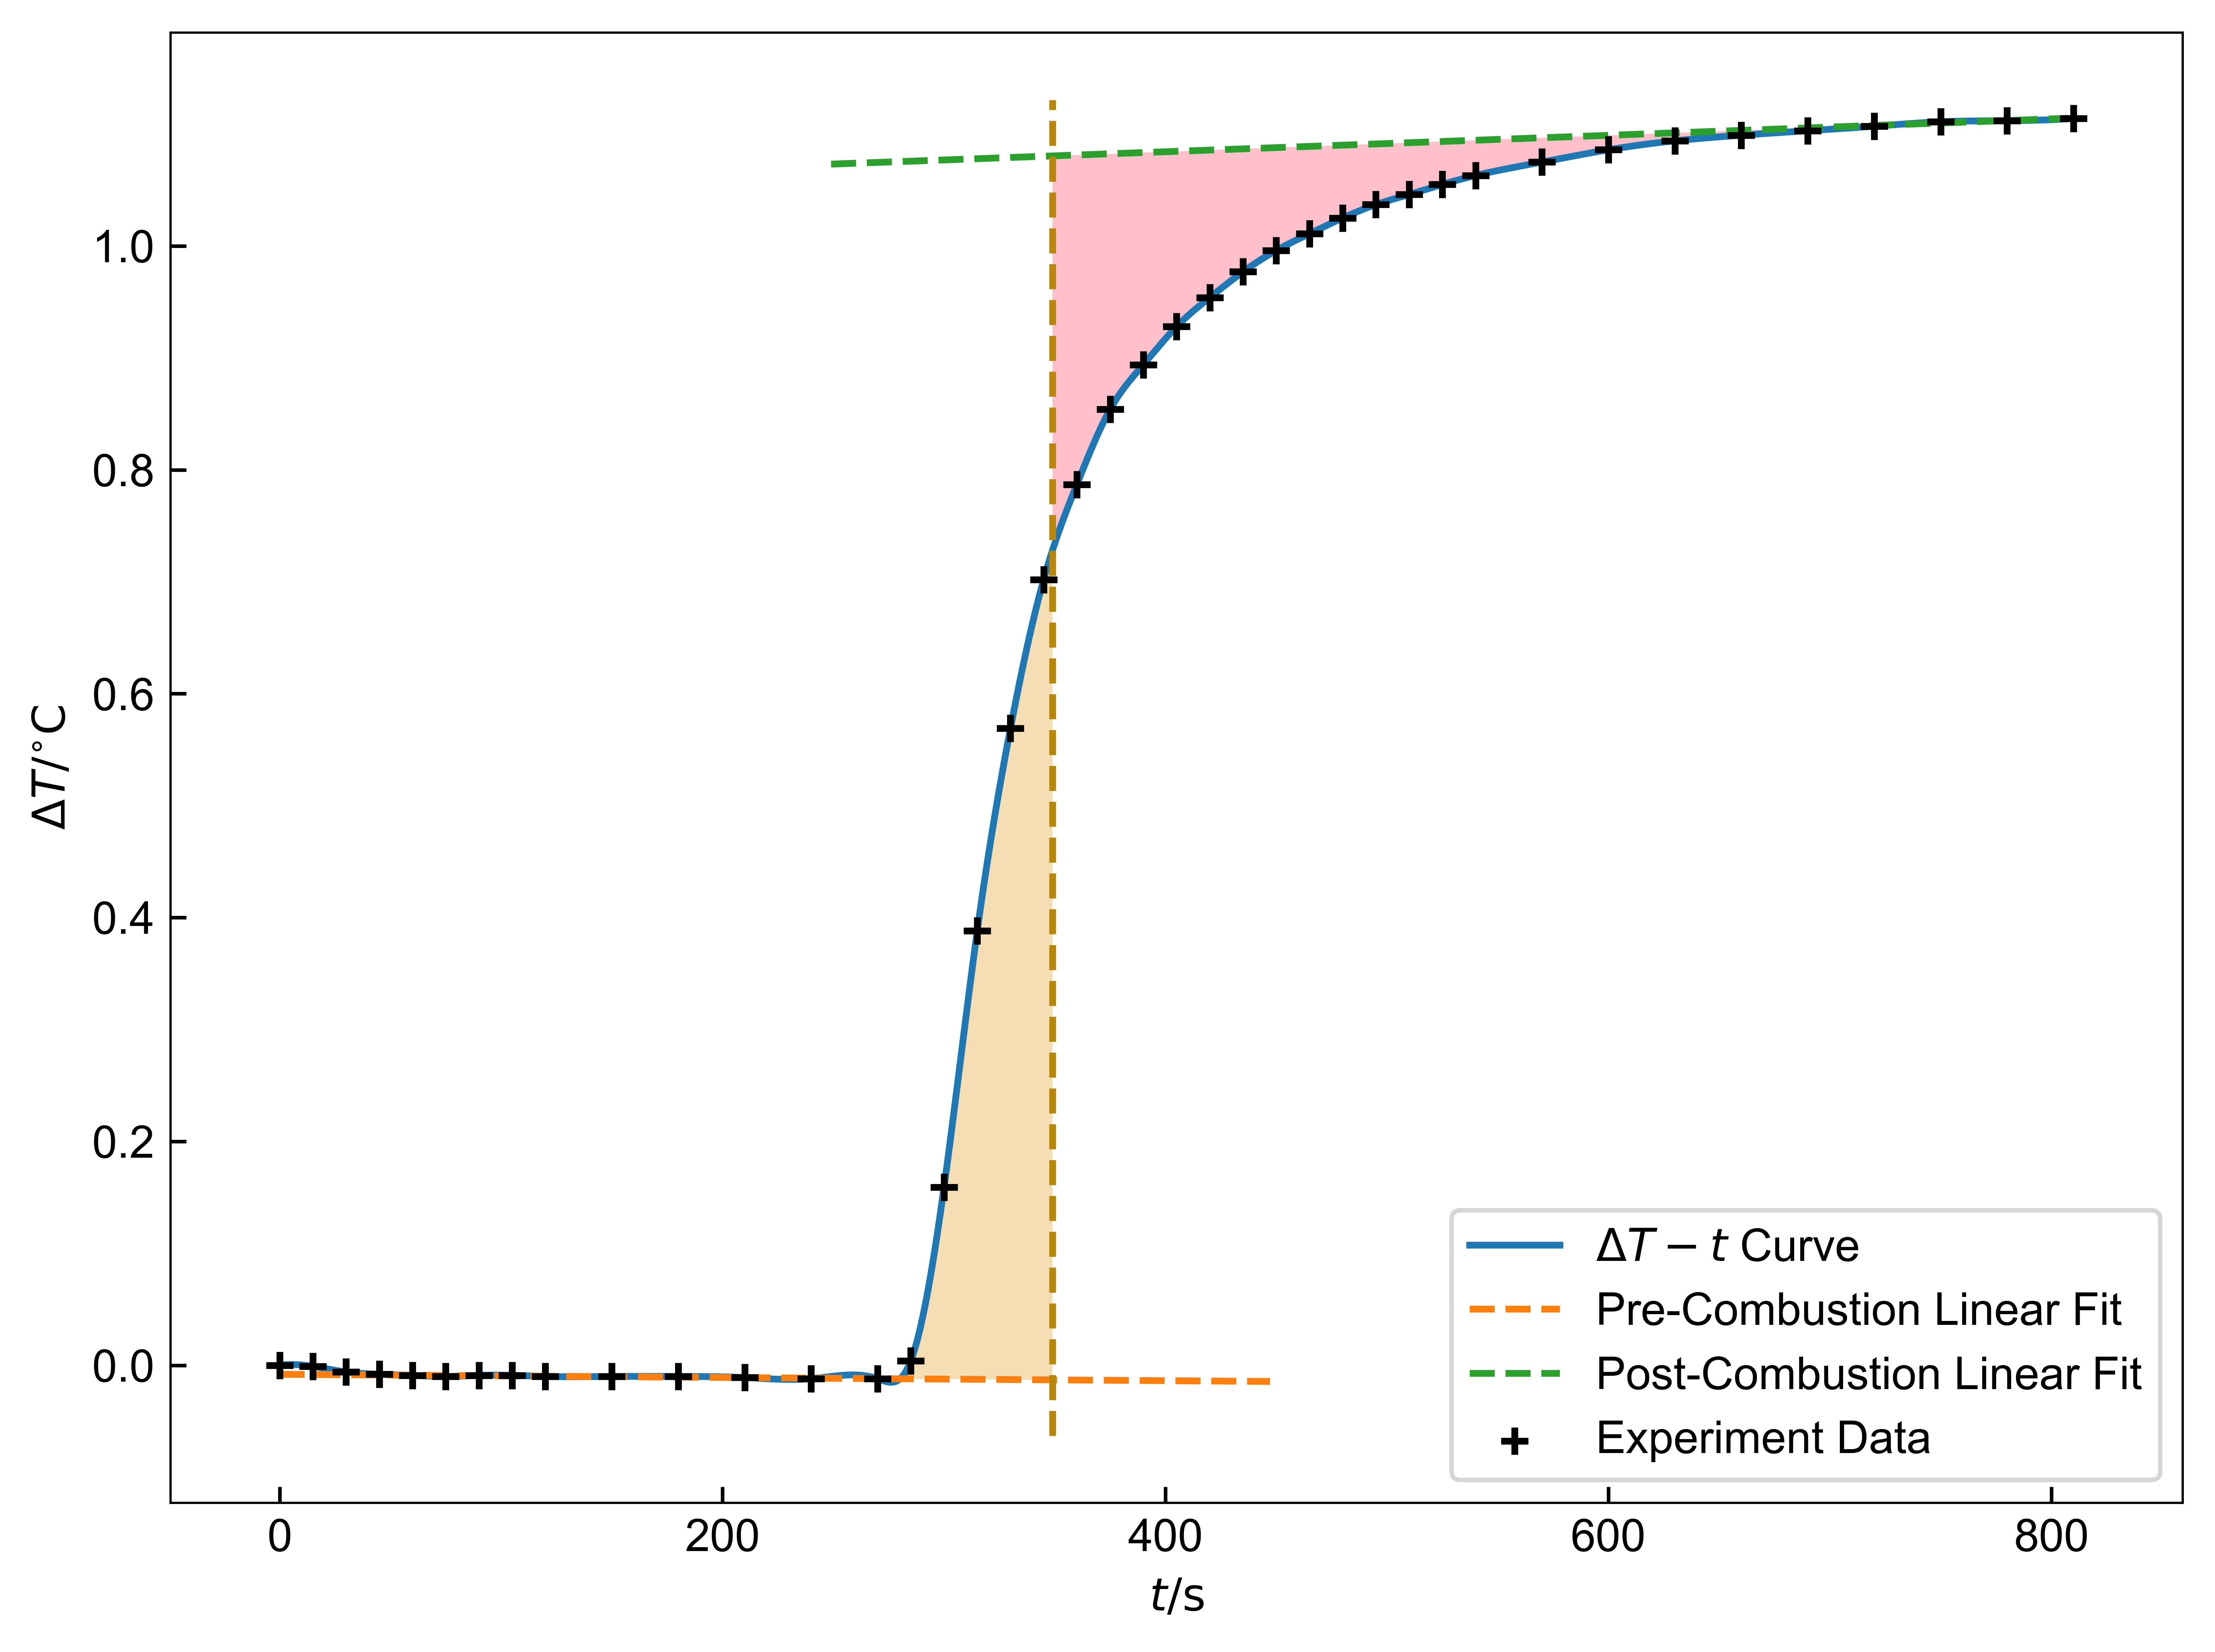
\includegraphics[width=0.7\textwidth]{2.jpg}
	\bicaption{蔗糖燃烧过程$\Delta T-t$曲线及雷诺校正}{$\Delta T-t$ curve of sucrose combustion process and Renolds correction}
\end{figure}
\par
测定前期拟合直线的方程为
$$
\Delta T/{\rm ^{\circ}C} =-(1.4\pm 0.2)\times 10^{-5} \ \ t/{\rm s}-(8.1\pm 0.4)\times 10^{-3},\  \ R^{2}=0.8313
$$
测定末期拟合直线的方程为
$$
\Delta T/{\rm ^{\circ}C} =(7.3\pm 1.4)\times 10^{-5} \ \ t/{\rm s}+(1.05\pm 0.01),\  \ R^{2}=0.9308
$$
确定使得两部分面积相等的时间点
$$
t_{0}=348.99\ \ {\rm s}
$$
计算垂线$t=t_{0}$与测定前期拟合直线的交点对应的温差(因计算方法与3.1.1相同,故略去,下同)
$$
\Delta T_{1}=-(0.0130\pm 0.0008)\ \ {\rm ^{\circ}C}
$$
计算垂线$t=t_{0}$与测定末期拟合直线的交点对应的温差
$$
\Delta T_{2}=(1.08\pm 0.01)\ \ {\rm ^{\circ}C}
$$
因此,计算蔗糖燃烧过程放出热量致使体系温度升高的数值
$$
\Delta T_{0}=(1.09\pm 0.01)\ \ {\rm ^{\circ}C}
$$


 \subsection{数据处理结果与分析}
 \subsubsection{计算水当量}
仪器的量热器常数(水当量)$W$可由下式求算:
$$
W=\frac{-Q_{V}G-\Sigma q}{\Delta T_{0}}-DC_{\rm H_{2}O}
$$
其中,$\Delta T_{0}$为苯甲酸燃烧使体系温度升高的数值,由3.1.1知$\Delta T_{0}=(1.62\pm 0.01)\ \ {\rm ^{\circ}C}$;$G$为苯甲酸的质量,由2.2.1知$G=m-m^{\prime}=0.9044\ \ {\rm g}$;$C_{\rm H_{2}O}$为水的比热容,随温度变化不大,查阅\textit{CRC Handbook of Chemistry and Physics}\citealp{crc},取$298.15\ \ {\rm K}$时的数据$C_{\rm H_{2}O}=4.184\ \ {\rm J\cdot g^{-1}\cdot K^{-1}}$;$D$为加入水的质量,考虑实验过程中室温$T=18.6\ \ {\rm ^{\circ}C}$,苯甲酸燃烧过程中温度变化不大,取$20\ \ {\rm ^{\circ}C}$时水的密度$\rho=0.9989\ \ {\rm kg\cdot m^{-3}}$,计算
$$
D=\rho V=0.9989\ \ {\rm kg\cdot m^{-3}} \times 3000\ \ {\rm mL}=2997\ \ {\rm g}
$$
$Q_{V}$为苯甲酸的恒容燃烧热,假设量热器内气体具有理想行为,则
$$
Q_{V}=Q_{P}-\frac{\Delta n RT}{M}
$$
苯甲酸燃烧的反应方程式
$$
\ce{C6H5COOH(s) +  15/2 O2(g) -> 7 CO2(g) + 3 H2O(l)}
$$
故$\Delta n=-0.5\ \ {\rm mol}$;苯甲酸的恒压燃烧热$Q_{P}=-26460\ \ {\rm J\cdot g^{-1}}$,从\textbf{图1}读取垂线$t=t_{0}$与$\Delta T-t$曲线的交点对应的温差$\Delta T=1.12\ \ {\rm ^{\circ}C}$,取$T=(291.75+1.12)\ \ {\rm K}=292.87\ \ {\rm K}$,故计算
$$
Q_{V}=(-26460+\frac{0.5\times 8.3145 \times 292.87}{122.118})\ \ {\rm J\cdot g^{-1}}=-26450\ \ {\rm J\cdot g^{-1}}
$$
$\Sigma q$为燃烧丝(镍丝)及棉线燃烧热的校正值,由于棉线的恒容燃烧热$Q_{V, {\rm Cotton}}=-16736\ \ {\rm J\cdot g^{-1}}$,镍丝的恒容燃烧热$Q_{V, {\rm Ni}}=-3243\ \ {\rm J\cdot g^{-1}}$,由2.2.1知棉线质量$m^{\prime}=0.0164\ \ {\rm g}$,发生燃烧的镍丝质量$m_{\rm Ni}=m_{0}-m_{1}=0.0014\ \ {\rm g}$,故计算
$$
\Sigma q=Q_{V, {\rm Cotton}} \ \ m^{\prime}+Q_{V, {\rm Ni}} \ \ m_{\rm Ni}=-279\ \ {\rm J}
$$
根据以上各项数据,计算量热计常数
$$
W=\frac{-Q_{V}G-\Sigma q}{\Delta T_{0}}-DC_{\rm H_{2}O}=(\frac{26450\times 0.9044+279}{1.62}-2997\times 4.184)\ \ {\rm J\cdot K^{\-1}}=2399\ \ {\rm J\cdot K^{-1}}
$$
量热计常数$W$的不确定度
$$
\sigma_{W}=\frac{(-Q_{V}G-\Sigma q)\sigma_{\Delta T_{0}}}{(\Delta T_{0})^{2}}=\frac{(26450\times 0.9044+279)\times 0.01}{1.62^{2}}=92\ \ {\rm J\cdot K^{-1}}
$$
故
$$
W=(2399\pm 92)\ \ {\rm J\cdot K^{-1}}=(2.40\pm 0.09)\ \ {\rm kJ\cdot K^{-1}}
$$
\subsubsection{计算蔗糖的燃烧热}
蔗糖的恒容燃烧热$Q_{V}$可由下式求算:
$$
Q_{V}=-\frac{(W+DC_{\rm H_{2}O})\Delta T_{0}+\Sigma q}{G}
$$
其中,$\Delta T_{0}$为蔗糖燃烧使体系温度升高的数值,由3.1.2知$\Delta T_{0}=(1.09\pm 0.01)\ \ {\rm ^{\circ}C}$;$G$为蔗糖的质量,由2.2.2知$G=m-m^{\prime}=0.9677\ \ {\rm g}$;$D$为加入水的质量,由3.2.1知$D=2997\ \ {\rm g}$;$C_{\rm H_{2}O}$为水的比热容,由3.2.1知$C_{\rm H_{2}O}=4.184\ \ {\rm J\cdot g^{-1} \cdot K^{-1}}$;$W$为量热计常数,由3.2.1知$W=(2399\pm 92)\ \ {\rm J\cdot K^{-1}}$;$\Sigma q$为燃烧丝(镍丝)及棉线燃烧热的校正值,由2.2.2知棉线质量$m^{\prime}=0.0185\ \ {\rm g}$,发生燃烧的镍丝质量$m_{\rm Ni}=m_{0}-m_{1}=0.0019\ \ {\rm g}$,故计算
$$
\Sigma q=Q_{V, {\rm Cotton}} \ \ m^{\prime}+Q_{V, {\rm Ni}} \ \ m_{\rm Ni}=-316\ \ {\rm J}
$$
根据以上各项数据,计算蔗糖的恒容燃烧热
$$
Q_{V}=\frac{-(2399+2997\times 4.184)\times 1.09+316}{0.9677}\ \ {\rm J\cdot g^{-1}}=-16500\ \ {\rm J\cdot g^{-1}}
$$
不确定度
$$
\sigma_{Q_{V}}=\frac{1}{G}\sqrt{((W+DC_{\rm H_{2}O})\sigma_{\Delta T_{0}})^{2}+(\Delta T_{0}\sigma_{W})^{2}} \ \ {\rm J\cdot g^{-1}}=186\ \ {\rm J\cdot g^{-1}}
$$
故蔗糖的恒容燃烧热
$$
Q_{V}=-(16500\pm 186)\ \ {\rm J\cdot g^{-1}}=-(16.5\pm 0.2)\ \ {\rm kJ\cdot g^{-1}}
$$
记蔗糖的恒压燃烧热为$Q_{P}$,假设量热器内气体具有理想行为,则
$$
Q_{P}=Q_{V}+\frac{\Delta n RT}{M}
$$
蔗糖燃烧的反应方程式
$$
\ce{C12H22O11(s) +  12 O2(g) -> 12 CO2(g) + 11 H2O(l)}
$$
故$\Delta n=0$,蔗糖的恒压燃烧热
$$
Q_{P}=Q_{V}=-(16500\pm 186)\ \ {\rm J\cdot g^{-1}}=-(16.5\pm 0.2)\ \ {\rm kJ\cdot g^{-1}}
$$
蔗糖的摩尔质量$M=342.30\ \ {\rm g\cdot mol^{-1}}$,故
$$
\Delta_{c}H_{m}=Q_{P}M=-(5648\pm 64)\ \ {\rm kJ\cdot mol^{-1}} 
$$
查阅\textit{CRC Handbook of Chemistry and Physics}\citealp{crc},知蔗糖的标准摩尔燃烧热
$$
\Delta_{c}H^{\circ}_{m}=-5640.9\ \ {\rm kJ\cdot mol^{-1}}
$$
故实验所测定的蔗糖燃烧热与文献参考值较为接近,相对误差为
$$
\xi=\frac{-5648+5640.9}{-5640.9}\times 100\%=0.12\%
$$
即实验测得蔗糖燃烧热的绝对值略偏大。

\vbox{}
 	 \section{讨论与结论}
		\subsection{实验讨论}
 			\subsubsection{误差分析:加入水量的误差}
 		实验过程中,分别用$2000\ \ {\rm mL}$容量瓶、$1000\ \ {\rm mL}$容量瓶向量热器中加入$2000\ \ {\rm mL}$、$1000\ \ {\rm mL}$去离子水。取容量瓶的不确定度为$0.1\%$,则加入水的体积的不确定度为
 		$$
 		\sigma_{V}=3000\ \ {\rm mL} \times 0.1\% =3 \ \ {\rm mL}
 		$$
 		由此带来加入水的质量的不确定度
 		$$
 		\sigma_{D}=\rho \sigma_{V}=2.9967\ \ {\rm g}
 		$$
 		由此带来量热计常数$W$的不确定度
 		$$
 		\sigma_{W}=C_{\rm H_{2}O}\sigma_{D}=12.5\ \ {\rm J\cdot K^{-1}}
 		$$
 		相比3.2.1计算得到的$W$的不确定度$\sigma_{W}=92\ \ {\rm J\cdot K^{-1}}$,加入水量的误差带来的$W$的不确定度虽显著小于前者,但仍是不可忽略的,为量热计常数$W$的测定引入了相当程度的误差。但加入水量的误差对于蔗糖的恒容燃烧热$Q_{V}$的影响较小,这是因为若两次加水操作相同,可以合理假设加入水量的误差主要来源于容量瓶中有水残余等系统误差,则两次加水的系统误差在$Q_{V}$的计算式中相互抵消,因此对$Q_{V}$的影响较小。
 	\subsubsection{误差分析:实验条件偏离标准态的系统误差}
 	蔗糖燃烧热的文献参考值$\Delta_{c}H^{\circ}_{m}=-5640.9\ \ {\rm kJ\cdot mol^{-1}}$在标准态下测得,而实验测定蔗糖燃烧热过程中,实验条件偏离标准态,引入了一定的系统误差。\par 
 	实验过程中,温度偏离标准态$298.15\ \ {\rm K}$,考虑体系压强变化不大,近似以恒压热容$C_{P}$代替恒容热容$C_{V}$,查阅\textit{CRC Handbook of Chemistry and Physics}\citealp{crc}知\ce{H2O}的恒压热容$C_{P}=75.3\ \ {\rm J\cdot K^{-1} \cdot mol^{-1}}$,\ce{O2}的恒压热容$C_{P}=29.4\ \ {\rm J\cdot K^{-1} \cdot mol^{-1}}$,蔗糖的恒压热容$C_{P}=430\ \ {\rm J\cdot K^{-1} \cdot mol^{-1}}$,\ce{CO2}的恒压热容$C_{P}=37.1\ \ {\rm J\cdot K^{-1} \cdot mol^{-1}}$,因此对于整个反应:
 	$$\Delta C_{P}=(11\times 75.3+12\times 37.1-12\times 29.4-430)\ \ {\rm J\cdot K^{-1} \cdot mol^{-1}}=491\ \ {\rm J\cdot K^{-1} \cdot mol^{-1}}
 	$$
 	近似取反应温度与标准态$298.15\ \ {\rm K}$的温度差$\Delta T=5\ \ {\rm K}$,则温度偏离标准态的修正
 	$$
 	\Delta_{c}H_{m}-\Delta_{c}H^{\circ}_{m}=\Delta C_{P} \Delta T=2.4\ \ {\rm kJ\cdot mol^{-1}}
 	$$
	该项修正远小于蔗糖摩尔燃烧热的测定值,可以忽略不计。
		\subsubsection{误差分析:部分固体脱落带来误差}
		在压片操作及转移过程中,由于蔗糖较为松散,可以观察到不断有碎屑脱落,导致称量得到的蔗糖质量与实际参与燃烧的蔗糖质量有较大差别。不妨估算蔗糖碎屑脱落带来的蔗糖质量的不确定度$\Delta G=0.05\ \ {g}$,因而导致的
		$$
		\Sigma_{Q_{V}}=292\ \ {\rm kJ\cdot mol^{-1}}
		$$
		影响极其显著。因此,可以判断蔗糖固体脱落为蔗糖燃烧热的测定带来了极大的实验误差。
 			
 		



 	 \subsection{实验结论}
 	 本实验通过氧弹式量热计中苯甲酸和蔗糖的恒容燃烧,经雷诺校正及热力学计算得到量热计常数$W=(2.40\pm 0.09)\ \ {\rm kJ\cdot K^{-1}}$,蔗糖的恒容燃烧热及恒压燃烧热$Q_{P}=Q_{V}=-(16.5\pm 0.2)\ \ {\rm kJ\cdot g^{-1}}$,换算得$\Delta_{c}H_{m}=-(5648\pm 64)\ \ {\rm kJ\cdot mol^{-1}}$,与文献值的偏差$\xi=0.12\%$,并对加入水量误差、实验条件偏离标准态误差、固体脱落误差等进行了分析。\par 
 	 经过误差分析,可以发现主要的误差来源为部分蔗糖固体脱落带来的误差。


 

   

\vbox{}

\bibliographystyle{achemso}
\bibliography{b}



\end{document}